\section{Назначение и структура модуля sc-core}

Модуль sc-core – это набор библиотек и программ, которые составляют
ядро обработки sc-текстов. В него входят следующие динамические
библиотеки:
\begin{itemize}
\item libsys : библиотека, обеспечивающая независимость от
  операционной системы;
\item libtgf : библиотека обработки формата TGF (Transfer Graph Format);
\item libsc : библиотека моделирования sc-памяти;
\item libpm : библиотека процессорного модуля для обработки sc-текстов
  (например, она включает scp-интерпретатор и навигационно-поисковую
  машину);
\item librgp : библиотека удаленного подключения к sc-памяти по
  протоколу RGP (Remote Graph Protocol).
\end{itemize}

Также модуль sc-core включает следующие программы:
\begin{itemize}
\item start-pm : средство запуска процессорного модуля из консоли;
\item dumptgf : утилита для просмотра TGF-файлов в человеко-читаемой
  форме;
\item scs2tgf : транслятор sc.s-текстов в формат TGF.
\end{itemize}

Как вы уже знаете, при установке инсталлятор модуля sc-core создает
переменную среды \verb+SC_CORE_HOME+, которая в качестве своего значения
будет иметь путь к корневой папке установленного модуля. Если вы
заглянете в эту папку, то сможете увидеть следующую структуру папок и
файлов (пути даются относительно значения переменной окружения
\verb+SC_CORE_HOME+):
\begin{itemize}
\item \verb|bin/| : бинарные файлы библиотек и программ. В этой директории
  динамические библиотеки для отладочной версии приложения имеют в
  конце имени букву «d» (сравните, libSCd.dll и libSC.dll);
\item \verb|doc/| : doxygen-документация на английском языке по модулю sc-core;
\item \verb|examples/| : примеры использования модуля:
  \begin{itemize}
  \item \verb|wave_find_path/| : С++-пример использования библиотеки
    sc-памяти libsc на основе алгоритма поиска одного из минимальных
    путей в неориентированном графе;
  \item \verb|fs_repo_src/| : SCP-пример на основе алгоритма поиска одного из
    минимальных путей в неориентированном графе;
  \end{itemize}
\item \verb|include/| : содержит директории с заголовочными файлами для всех библиотек
  модуля;
\item \verb|lib/| : библиотеки импорта для всех динамических библиотек модуля
  В этой директории библиотеки импорта для отладочной версии
  динамической библиотеки имеют в конце имени букву «d» (сравните,
  libSCd.lib и libSC.lib);
\item \verb|share/| : содержит дополнительные необходимые ресурсы для работы
  модуля, которые нельзя отнести ни в одну из уже описанных
  директорий.
\end{itemize}

Из всего описанного выше в контексте данного руководства нас будет
интересовать библиотека моделирования sc-памяти libsc и пример ее
использования \verb|wave_find_path|. В ходе дальнейшего разговора мы сначала
будем рассматривать основные понятия, структуру и классы библиотеки
libsc, а затем перейдем к более конкретному рассмотрению примера
использования этой библиотеки.

\section{Библиотека моделирования sc-памяти – libsc}

В данном разделе мы рассмотрим библиотеку моделирования sc-памяти в
объеме, необходимом для выполнения это этапа расчетной работы.

\subsection{Общие сведения}

Библиотека моделирования sc-памяти написана на языке C++, поэтому в
этом разделе мы будем рассматривать в основном классы для
моделирования sc-памяти и их методы, а также некоторые функции попадут
в поле нашего зрения. Однако сейчас давайте рассмотрим файлы и
директории из модуля sc-core, которые имеют отношение к библиотеке. И
так, приступим (пути даются относительно значения переменной окружения
\verb|SC_CORE_HOME|):
\begin{itemize}
\item \verb|bin/libSCd.dll| : debug-версия динамической библиотеки
  моделирования sc-памяти;
\item \verb|bin/libSC.dll| : release-версия динамической библиотеки
  моделирования sc-памяти;
\item \verb|lib/libSCd.lib| : библиотека импорта для динамической библиотеки
  libSCd.dll;
\item \verb|lib/libSC.lib| : библиотека импорта для динамической библиотеки
  libSC.dll;
\item \verb|doc/sc-core/| : общая doxygen-документация по модулю
  sc-core, в том числе и по рассматриваемой библиотеке libsc;
\item \verb|include/libSC/| : заголовочные файлы рассматриваемой
  библиотеки;
\item \verb|examples/wave_find_path| : пример использования
  рассматриваемой библиотеки.
\end{itemize}

Библиотека libsc зависит от библиотеки обработки формата TGF libtgf, к
которой относятся следующие директории и папки (пути даются
относительно значения переменной окружения \verb|SC_CORE_HOME|):

\begin{itemize}
\item \verb|bin/libTGFd.dll| : debug-версия динамической библиотеки
  libtgf (она необходима для работы с libSCd.dll);
\item \verb|bin/libTGF.dll| : release-версия динамической библиотеки
  libtgf (она необходима для работы с libSC.dll);
\item \verb|include/libTGF/| : заголовочные файлы библиотеки libtgf;
\end{itemize}

Теперь перейдем к непосредственному описанию библиотеки libsc.

\subsection{Сегментная модель sc-памяти}

Когда вы занимались формализацией на SCg по курсу МОИС, то считали,
что sc-элементы с одинаковыми идентификаторами должны
склеиться. Однако в реализации sc-памяти используется сегментная
модель и поэтому всё несколько сложнее.

В сегментной модели вся память разбивается на sc-сегменты, где каждый
sc-элемент принадлежит ровно одному сегменту. Уникальность
идентификаторов sc-элементов имеет место только в рамках
sc-сегмента. Сами sc-сегменты могут организовываться в рамках
sc-директории. Проиллюстрирую на конкретной структуре sc-памяти:

\begin{itemize}
\item /: корневая sc-директория, которая всегда существует
  
  \begin{itemize}
  \item \verb|graph_theory/|: sc-директория, которая содержит базу знаний по
    теории графов
    \begin{itemize}
    \item \verb|keynode|: sc-сегмент, который содержит ключевые
      узлы базы знаний по теории графов
      \begin{itemize}
      \item \idtf{графовая структура}
      \item \idtf{вершина\_}
      \item \idtf{связка\_}
      \item \idtf{неориентированный граф}
      \item \idtf{ребро\_} и т.д.
      \end{itemize}
    \end{itemize}

  \item \verb|tmp/|: содержит sc-сегменты для временной обработки
    sc-конструкций
    \begin{itemize}
    \item \verb|wave_find_path| : временный sc-сегмент для работы алгоритма
      поиска одного из минимальных путей в неориентированном графе
    \end{itemize}

  \item \verb|proc/|: содержит системные sc-сегменты;
    \begin{itemize}
    \item \verb|keynode|: sc-сегмент, который содержит системные ключевые
      узлы
      \begin{itemize}
      \item \idtf{1\_}
      \item \idtf{2\_} и т.д.
      \end{itemize}
    \end{itemize}
  \end{itemize}
\end{itemize}

Такая структура sc-директорий и sc-сегментов аналогична структуре
папок и файлов на файловой системе. Аналогом файла является
sc-сегмент, а аналогом содержимого файла является sc-конструкции. В
сегментной модели любой объект (sc-директория, sc-сегмент, sc-элемент)
может быть однозначно идентифицирован при помощи строки особого вида,
которая по историческим причинам называется URI (Universal Resource
Identifier). Формат URI аналогичен формату пути к папке или файлу на
файловых системах Unix-подобных операционных систем. Вот некоторые
примеры URI:

\begin{itemize}
\item \verb|/|: URI sc-директории
\item \verb|/graph_theory/keynode| : URI sc-сегмента
\item \verb|/graph_theory/keynode/вершина_| : URI sc-элемента
\end{itemize}

Адресация sc-элементов с использованием URI удобна для человека, но
неудобна для компьютера, поэтому существует понятие
sc-адреса. SC-адрес – это некоторое число, которое однозначно
идентифицирует sc-элемент в сегментной модели sc-памяти. С
использованием sc-адресов sc-элементов ведется их обработка в рамках
sc-сессии. SC-сессия - это логически единая последовательность
операций над некоторой областью sc-памяти (sc-директориями,
sc-сегментами, sc-элементами). Для того, чтобы получить доступ к
данным sc-сегмента, нужный sc-сегмент должен быть открыт в рамках
используемой sc-сессии. Существует особый вид sc-сессии, который
называется системная sc-сессия, в рамках которой все существующие
sc-сегменты всегда открыты.

Я думаю, что читатель уже получил общие сведения о том, что такое
сегментная модель, sc-директория, sc-сегмент, URI, sc-адрес,
sc-сессия, поэтому в следующем разделе я начну рассматривать
практические вопросы использования библиотеки моделирования sc-памяти.

\subsection{Начало работы с библиотекой libsc}
\label{sec:Begin_with_libsc}

В прошлом разделе мы рассмотрели логическое устройство сегментной
модели sc-памяти, а теперь проведем аналогию с текущей реализацией на
языке программирования С++.

Понятию sc-сегмента в библиотеке libsc соответствует класс
\lstinline{sc_segment}, который описан в файле
\verb|sc_segment.h|. Понятию sc-адреса соответствует
\lstinline{typedef sc_addr} из заголовочного файла \verb|sc_types.h|,
а sc-сессии – класс \lstinline{sc_session} из \verb|libsc.h|. Для
представления URI и идентификаторов sc-элементов используется
\lstinline{typedef sc_string} (это просто другое имя для
\lstinline{std::string}), объявленный в \verb|sc_types.h|. Чтобы
начать работу со всеми этими типами, достаточно подключить только один
заголовочный файл, а именно \verb|libsc.h|, потому что в него включены
и \verb|sc_segment.h|, и \verb|sc_types.h|.

Работа с объектами классов \lstinline{sc_session} и
\lstinline{sc_segment} всегда ведется через указатель на объект,
поэтому методы и функции, которые возвращают указатель на объекты этих
классов, могут возвращать \lstinline{0} или \lstinline{NULL}, чтобы
показать наличие ошибки в процессе выполнения. Если в тексте ниже я
буду писать о работе с объектами классов \lstinline{sc_session} и
\lstinline{sc_segment}, то это почти всегда надо понимать, как работу
с такими объектами через указатель.

Рассмотрим, как обстоят дела в этом плане с типом
\lstinline{sc_addr}. В \verb|sc_types.h| он объявлен следующим образом:
\begin{lstlisting}
  typedef sc_global_addr *sc_addr;
\end{lstlisting}

Как видно из приведенного выше объявления, \lstinline{sc_addr} – это
указатель на класс \lstinline{sc_global_addr}. Поэтому методы и
функции, которые возвращают \lstinline{sc_addr}, могут возвращать
\lstinline{0}, \lstinline{NULL} или \lstinline{SCADDR_NIL} (это
\lstinline{define} для \lstinline{0}), чтобы показать наличие ошибки в
процессе выполнения. В отличие от \lstinline{sc_session} и
\lstinline{sc_segment}, с типом \lstinline{sc_addr} мы работаем без
указателя, потому что \lstinline{sc_addr} – это и так указатель
(просто другое имя для указателя на
\lstinline{sc_global_addr}). Напоследок об \lstinline{sc_addr} стоит
сказать следующее:
\begin{itemize}
\item для переменных этого типа можно использовать операторы
  \lstinline{==} и \lstinline{!=}, чтобы проверить идет работа с одним
  и тем же sc-элементом или с разными;
\item у \lstinline{sc_global_addr} есть открытое поле
  \lstinline{sc_global_addr::seg}, которое позволяет получить
  sc-cегмент, в котором находится адресуемый sc-элемент;
\item если в дальнейшем будет идти речь о работе с sc-элементами, то
  это значит, что речь идет о работе с соответствующими им
  sc-адресами.
\end{itemize}

Предыдущий текст должен был вас уже утомить, поэтому разбавим этот
раздел примерами кода. Для начала работы с моделью sc-памяти ее надо
инициализировать, это можно сделать вот так:

\begin{lstlisting}[texcl]
  #include <libsc.h>

  // $\dots$
  // Инициализируем sc-память при помощи функции \verb|libsc_init|.
  // Она вернет системную sc-сессию.
  // 
  sc_session *system = libsc_init();
\end{lstlisting}

Теперь необходимо инициализировать системные ключевые узлы (например,
\idtf{1\_}, \idtf{2\_} и др.). Все системные ключевые узлы объявлены в
заголовочном файле \verb|pm_keynodes.h| и инициализируются функцией
\lstinline{pm_keynodes_init}:

\begin{lstlisting}[texcl]
  #include <pm_keynodes.h>

  // $\dots$
  // Ключевые узлы будут созданы в sc-сегменте "/proc/keynode".
  // Например:
  //  - для работы с ключевым узлом \idtf{1\_} можно использовать имя \verb|N1_|
  //  - для работы с ключевым узлом \idtf{2\_} можно использовать имя \verb|N2_|
  //  - закономерность очевидна $\dots$
  //
  pm_keynodes_init(system);
\end{lstlisting}

В принципе уже можно работать с sc-памятью через системную sc-сессию
\lstinline{system}, но в идеале лучше работать через пользовательскую
sc-сессию:

\begin{lstlisting}[texcl]
  // Получим пользовательскую sc-сессию при помощи функции \verb|libsc_login|.
  //
  sc_session *session = libsc_login();

  // При помощи метода \verb|sc_session::open_segment| по URI "/proc/keynode"
  // откроем в нашей пользовательской sc-сессии sc-сегмент системных 
  // ключевых узлов.
  //
  session->open_segment(“/proc/keynode”);
\end{lstlisting}

Теперь создадим уникальный sc-сегмент для исследования работы
sc-памяти:

\begin{lstlisting}[texcl]
  // Этот заголовочный файл содержит функции, которые облегчают работу с 
  // sc-сегментами.
  #include <segment_utils.h>
  
  // $\dots$
  // Создадим уникальный sc-сегмент с использованием \verb|create_unique_segment|
  // и URI этого sc-сегмента будет начинатся с "/tmp/test".
  // 
  sc_segment *segment = create_unique_segment(session, “/tmp/test”);

  // Созданный при помощи sc-сессии session sc-сегмент будет автоматический
  // открыт в ней.
  //
\end{lstlisting}

Пользовательская sc-сессия \lstinline{session} и созданный sc-сегмент
\lstinline{segment} будут использоваться во всех дальнейших примерах
без какого-то явного объявления.

После окончания необходимой работы sc-память нужно почистить:
\begin{lstlisting}[texcl]
  // Удалим созданный sc-сегмент seg при помощи метода \verb|sc_session::unlink|
  // Метод \verb|sc_segment::get_full_uri| возвращает URI sc-сегмента.
  //
  session->unlink(segment->get_full_uri());

  // Закроем пользовательскую sc-сессию.
  //
  session->close();

  // Деинициализируем sc-память.
  //
  libsc_deinit();

  // Обратите внимани на то, что явно при помощи оператора \verb|delete| никакая 
  // память не освобождается. При работе с типами \verb|sc_session|, \verb|sc_segment|,
  // \verb|sc_addr| память явно освобождать не надо.
  //
\end{lstlisting}

Перед тем, как мы будем рассматривать операции генерации и поиска в
sc-памяти, вам еще нужно познакомиться со способом задания типа
sc-элементов, поэтому переходим к следующему разделу.

\subsection{Тип sc-элемента}

Для задания типа sc-элемента в библиотеке libsc используется С++-тип
\lstinline{sc_type}, который объявлен в файле
\verb|sc_types.h|. Значение типа \lstinline{sc_type} – это просто
число, которое является результатом операции побитового ИЛИ некоторых
числовых констант. Каждая из числовых констант задает значение
свойства из заранее определенного диапазона. Для выполнения расчетной
работы вам достаточно знать о следующих свойствах:

\begin{itemize}
\item Структурный тип sc-элемента. Используемые числовые константы
  С++:
  \begin{itemize}
  \item \lstinline{SC_UNDF}: sc-элемент неопределенного типа;
  \item \lstinline{SC_ARC}: sc-дуга;
  \item \lstinline{SC_NODE}: sc-узел.
  \end{itemize}

\item Константность sc-элемента. Используемые числовые константы С++:
  \begin{itemize}
  \item \lstinline{SC_CONST}: константность;
  \item \lstinline{SC_VAR}: переменность;
  \item \lstinline{SC_METAVAR}: метапеременность.
  \end{itemize}

\item Нечеткость sc-дуги. Используемые числовые константы С++:
  \begin{itemize}
  \item \lstinline{SC_POS}: позитивность;
  \item \lstinline{SC_NEG}: негативность;
  \item \lstinline{SC_FUZ}: нечеткость.
  \end{itemize}
\end{itemize}

С использованием описанных выше числовых констант, например,
константный sc-узел можно задать как \lstinline{SC_NODE|SC_CONST}, а
позитивную константную sc-дугу как
\lstinline{SC_ARC|SC_CONST|SC_POS}. В таблице~\ref{tab:SCgType2SCType}
приведены соответствующие значения типа \lstinline{sc_type} для всех
необходимых SCg-элементов. Обратите внимание, что на уровне библиотеки
libsc нет разницы в кодировании структурных типов SCg-элементов
(например, константный sc-атрибут и константное sc-отношение
кодируются как константный sc-узел).

\begin{table}[ht]
  \caption{Соответствие SCg-элемента значению типа sc\_type из libsc}
  \centering
  \begin{tabular}{|c|c|}
    \hline
	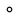
\includegraphics{images/4/scg2sc/undf_const} & \verb+SC_UNDF|SC_CONST+
    , \verb+SC_U_CONST+ \\
    
    \hline
    
\includegraphics{images/4/scg2sc/undf_var} & \verb+SC_UNDF|SC_VAR+, \verb+SC_U_VAR+ \\
    
    \hline
    
\includegraphics{images/4/scg2sc/undf_metavar} & \verb+SC_UNDF|SC_METAVAR+
    , \verb+SC_U_METAVAR+ \\
    
    \hline
    
\includegraphics{images/4/scg2sc/node_general_const}
    
\includegraphics{images/4/scg2sc/node_role_const}
    
\includegraphics{images/4/scg2sc/node_struct_const}
    
\includegraphics{images/4/scg2sc/node_concept_const}
    
\includegraphics{images/4/scg2sc/node_binary_const}
    & \verb+SC_NODE|SC_CONST+, \verb+SC_N_CONST+ \\
    
    \hline
    
\includegraphics{images/4/scg2sc/node_general_var}
    
\includegraphics{images/4/scg2sc/node_role_var}
    
\includegraphics{images/4/scg2sc/node_struct_var}
    
\includegraphics{images/4/scg2sc/node_concept_var}
    
\includegraphics{images/4/scg2sc/node_binary_var}
    & \verb+SC_NODE|SC_VAR+, \verb+SC_N_VAR+ \\
    
    \hline
    
\includegraphics{images/4/scg2sc/node_general_meta}
    
\includegraphics{images/4/scg2sc/node_role_meta}
    
\includegraphics{images/4/scg2sc/node_struct_meta}
    
\includegraphics{images/4/scg2sc/node_concept_meta}
    
\includegraphics{images/4/scg2sc/node_binary_meta}
    & \verb+SC_NODE|SC_METAVAR+, \verb+SC_N_METAVAR+ \\
    
    \hline
	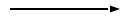
\includegraphics{images/4/scg2sc/arc_main} & \verb+SC_ARC|SC_CONST|SC_POS+
    , \verb+SC_A_CONST|SC_POS+ \\
    
    \hline
	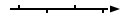
\includegraphics{images/4/scg2sc/pair_const_perm_fuz} & \verb+SC_ARC|SC_CONST|SC_FUZ+
    , \verb+SC_A_CONST|SC_FUZ+ \\
    
    \hline
	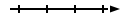
\includegraphics{images/4/scg2sc/pair_const_perm_neg} & \verb+SC_ARC|SC_CONST|SC_NEG+
    , \verb+SC_A_CONST|SC_NEG+ \\
    
    \hline
	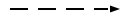
\includegraphics{images/4/scg2sc/pair_var_perm_pos} & \verb+SC_ARC|SC_VAR|SC_POS+
    , \verb+SC_A_VAR|SC_POS+ \\
    
    \hline
	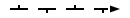
\includegraphics{images/4/scg2sc/pair_var_perm_fuz} & \verb+SC_ARC|SC_VAR|SC_FUZ+
    , \verb+SC_A_VAR|SC_FUZ+ \\
    
    \hline
	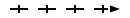
\includegraphics{images/4/scg2sc/pair_var_perm_neg} & \verb+SC_ARC|SC_VAR|SC_NEG+
    , \verb+SC_A_VAR|SC_NEG+ \\
    
    \hline
	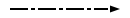
\includegraphics{images/4/scg2sc/pair_meta_perm_pos} & \verb+SC_ARC|SC_METAVAR|SC_POS+
    , \verb+SC_A_METAVAR|SC_POS+ \\
    
    \hline
	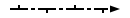
\includegraphics{images/4/scg2sc/pair_meta_perm_fuz} & \verb+SC_ARC|SC_METAVAR|SC_FUZ+
    , \verb+SC_A_METAVAR|SC_FUZ+ \\
    
    \hline
	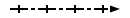
\includegraphics{images/4/scg2sc/pair_meta_perm_neg} & \verb+SC_ARC|SC_METAVAR|SC_NEG+
    , \verb+SC_A_METAVAR|SC_NEG+ \\
    
    \hline
  \end{tabular}
  \label{tab:SCgType2SCType}
\end{table}

Для получения и установки типа sc-элемента используются методы
\lstinline{sc_session::get_type} и
\lstinline{sc_session::change_type}. Более подробную информацию о них
можно найти в doxygen-документации.

Бинарные неориентированные (рис.~\ref{fig:Binary_unorient_pair}) и
ориентированные пары (рис.~\ref{fig:Binary_orient_pair}) в текущей
версии библиотеки libsc нельзя представить в виде атомарных элементов,
а представляются они так, как показано на
рисунках~\ref{fig:Unpack_binary_unorient_pair}~и~\ref{fig:Unpack_binary_orient_pair}
соответственно.

\begin{figure}[h!]
  \centering
  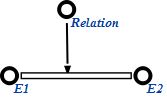
\includegraphics{images/4/scg2sc/Binary_unorient_pair}
  \caption{Бинарная неориентированная пара}
  \label{fig:Binary_unorient_pair}
\end{figure}

\begin{figure}[h!]
  \centering
  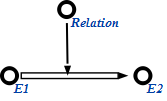
\includegraphics{images/4/scg2sc/Binary_orient_pair}
  \caption{Бинарная ориентированная пара}
  \label{fig:Binary_orient_pair}
\end{figure}

\begin{figure}[h!]
  \centering
  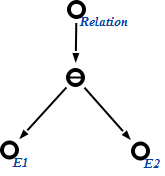
\includegraphics{images/4/scg2sc/Unpack_binary_unorient_pair}
  \caption{Кодирование бинарной неориентированной пары}
  \label{fig:Unpack_binary_unorient_pair}
\end{figure}

\begin{figure}[h!]
  \centering
  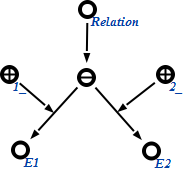
\includegraphics{images/4/scg2sc/Unpack_binary_orient_pair}
  \caption{Кодирование бинарной ориентированной пары}
  \label{fig:Unpack_binary_orient_pair}
\end{figure}

Как видно из приеденных рисунков бинарная неориентированная пара
представляется при помощи трех, а не одного sc-элемента. Бинарная
ориентированная пара представляется при помощи пяти sc-элементов, два
из которых (sc-узлы \idtf{1\_} и \idtf{2\_}) находятся в sc-сегменте
\verb|/proc/keynode| и являются ключевыми узлами.

В следующем разделе мы рассмотрим виды основных обрабатываемых
sc-конструкций.

\subsection{Основные обрабатываемые sc-конструкции}

В sc-памяти sc-элементы могут обрабатываться как поэлементно, так и
целыми группами. Можно выделить два вида таких групп sc-элементов.

Самой распространенной является трехэлементная sc-конструкция. Она
состоит из sc-узла и sc-элемента произвольного типа, которые связаны
sc-дугой. Пример частного случая трехэлементной sc-конструкции
приведен на рис.~\ref{fig:3_sc_constr} (обратите внимание на нумерацию
элементов). Этот частный случай трехэлементной sc-конструкции включает
в качестве первого элемента - константный sc-узел, второго элемента –
константную позитивную sc-дугу, в качестве третьего элемента -
константный sc-узел.

\begin{figure}[h!]
  \centering
  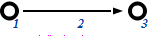
\includegraphics{images/4/3_sc_constr}
  \caption{Трехэлементная sc-конструкция}
  \label{fig:3_sc_constr}
\end{figure}

Не менее распространённой является пятиэлементная sc-конструкция,
частный случай которой приведен на рис.~\ref{fig:5_sc_constr}. Этот
частный случай пятиэлементной sc-конструкции включает в качестве 1-го
элемента – константный sc-узел, 2-го элемента – константную позитивную
sc-дугу, 3-го элемента – константный sc-узел, 4-го элемента -
константную позитивную sc-дугу, 5-го элемент – константный sc-узел.

\begin{figure}[h!]
  \centering
  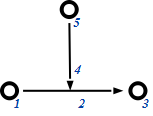
\includegraphics{images/4/5_sc_constr}
  \caption{Пятиэлементная sc-конструкция}
  \label{fig:5_sc_constr}
\end{figure}

Чаще всего пятиэлементная sc-конструкция используется, когда второй
элемент (sc-дуга) уточняется атрибутом, который является пятым
элементом пятиэлементной sc-конструкции.

\subsection{Генерация и удаление sc-конструкций в sc-памяти}

Для генерации одноэлементной sc-конструкции предназначен метод
\lstinline{sc_session::create_el}. Пример генерации константного
sc-узла (если sc-узел будет сгенерирован, то переменная получит в
качестве значения sc-адрес этого узла, иначе она получит в качестве
значения нулевой указатель):

\begin{lstlisting}[texcl]
sc_addr node = session->create_el(
    segment,      // sc-сегмент, в котором будет сгенерирован sc-элемент
    SC_N_CONST // тип sc-элемента
);
\end{lstlisting}

Давайте сгенерируем два константных sc-узла и присвоим им
идентификаторы при помощи метода \lstinline{sc_session::set_idtf} (для
получения идентификатора служит метод
\lstinline{sc_session::get_idtf}):

\begin{lstlisting}[texcl]
sc_addr e1 = session->create_el(segment, SC_N_CONST);
sc_addr e3 = session->create_el(segment, SC_N_CONST);

session->set_idtf(e1, "First");
session->set_idtf(e3, "Third");
\end{lstlisting}

В данной версии модели sc-памяти все sc-элементы всегда имеют
уникальный идентификатор, поэтому не удивляйтесь, если sc-элементы,
для которых вы не устанавливали идентификатор, будут иметь в качестве
него строки странного содержания. Это нормально. Вернемся к нашему
примеру.  Содержимое sc-сегмента segment после выполнение предыдущего
кода показано на рис.~\ref{fig:gen3_f_a_f_before}.

\begin{figure}
  \centering
  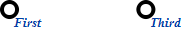
\includegraphics{images/4/gen/gen3_f_a_f_before}
  \caption{Содержимое sc-сегмент segment после генерации двух sc-узлов}
  \label{fig:gen3_f_a_f_before}
\end{figure}

В классе \lstinline{sc_session} есть специальный метод
\lstinline{gen3_f_a_f}, который генерирует второй элемент
трехэлементной sc-конструкции, если известны ее первый и третий
элементы. Его сигнатура выглядит следующим образом:
\begin{lstlisting}[texcl]
class sc_session
{
public:
    // $\dots$
    virtual sc_retval gen3_f_a_f(
        // sc-адрес 1-го элемент
        sc_addr e1,

        // по этому адресу поместить sc-адрес 2-го элемент
        sc_addr *e2,

        // sc-сегмент, в котором будет сгенерирован 2-ой элемент
        sc_segment *seg2,

        // тип 2-го элемента
        sc_type t2,

        // sc-адрес 3-го элемент
        sc_addr e3
    ) = 0;
    // $\dots$
};
\end{lstlisting}

Генерацию трехэлементной sc-конструкции с sc-узлами First и Third
можно провести следующим образом:
\begin{lstlisting}[texcl]
// переменная для sc-адреса 2-го элемента трехэлементной sc-конструкции.
sc_addr e2 = 0;

// Генерация sc-дуги между 1-ым и 3-им элементами.
session->gen3_f_a_f(
    // 1-ый элемент
    e1,

    // в e2 будет помещен sc-адрес 2-го элемента
    &e2,

    // sc-сегмент, в котором будет сгенерирован 2-ой элемент
    segment,

    // тип 2-ого элемента - константная позитивная sc-дуга
    SC_A_CONST|SC_POS,

    // 3-ий элемент
    e3
);
\end{lstlisting}

После выполнения приведенного выше кода содержимое sc-сегмента
\lstinline|segment| изменится так, как показано на
рис.~\ref{fig:gen3_f_a_f_after}.

\begin{figure}[h!]
  \centering
  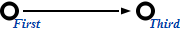
\includegraphics{images/4/gen/gen3_f_a_f_after}
  \caption{Пример генерации трехэлементной sc-конструкции}
  \label{fig:gen3_f_a_f_after}
\end{figure}

Но в некоторых случаях нам не надо получать sc-адрес второго элемента
при использовании метода \lstinline|sc_session::gen3_f_a_f|. В этом
случае можно в качестве второго аргумента этого метода передавать
нулевой указатель:

\begin{lstlisting}[texcl]
// Генерация sc-дуги между 1-ым и 3-им элементами.
session->gen3_f_a_f(
    // 1-ый элемент
    e1,

    // использован нулевой указатель,
    // а это значит что метод не будет возвращать sc-адрес
    // 2-го элемента трехэлементной sc-конструкции
    0,

    // sc-сегмент, в котором будет сгенерирован 2-ой элемент
    segment,

    // тип 2-ого элемента - константная позитивная sc-дуга
    SC_A_CONST|SC_POS,

    // 3-ий элемент
    e3
);
\end{lstlisting}

Запомните этот прием передачи нулевого указателя, потому что он
используется во многих методах и функциях libsc, которые должны
возвращать более одного аргумента.

Теперь обратим внимание на возвращаемое значение метода
\lstinline|sc_session::gen3_f_a_f|. Оно имеет тип
\lstinline|sc_retval| (sc-код возврата) и является просто числом, по
которому можно определить код произошедшей ошибки. Тип
\lstinline|sc_retval| используется во многих методах и функция
библиотеки, и вам необходимо знать о следующих значения этого типа:


\begin{itemize}
\item Константа \lstinline|RV_OK| : функция или метод отработал
  успешно;
\item Константа \lstinline|RV_ERR_GEN| : в процессе работы функции или метода
  произошла ошибка;
\item Константа \lstinline|RV_THEN| : функция или метод сообщает о
  том, что необходим переход по then-ветке условного оператора;
\item Константа \lstinline|RV_ELSE_GEN| : функция или метод сообщает о
  том, что необходим переход по else-ветке условного оператора.
\end{itemize}

В случае успешного выполнения метод \lstinline|sc_session::gen3_f_a_f|
возвратит \lstinline|RV_OK|, а в случае неуспешного –
\lstinline|RV_ERR_GEN|. Проверки можно организовать следующим образом:
\begin{lstlisting}[texcl]
if (session->gen3_f_a_f(...) == RV_OK) {
    // Генерация прошла успешно
} else {
    // Возникла ошибка в процессе генерации
}

// Зная о том, что константа RV\_OK равна 0 можно
// организовать проверку следующим образом.
if (!session->gen3_f_a_f(...)) {
    // Генерация прошла успешно
} else {
    // Возникла ошибка в процессе генерации
}

// Зная о том, что код ошибки неравен 0 можно
// организовать проверку ошибочной ситуации следующим образом.
if (session->gen3_f_a_f(...)) {
    // Возникла ошибка в процессе генерации
}
\end{lstlisting}

Если вы не пишете какой-то специальный устойчивый код, то такие
проверки в алгоритме генерации делать нет необходимости, потому что
ошибочный код возврата метод \lstinline|sc_session::gen3_f_a_f|
возвращает в следующих случаях:
\begin{itemize}
\item не удалось выделить память под генерируемые элементы;
\item sc-сегмент, в котором происходит генерация 2-го элемент
  трехэлементной sc-конструкции закрыт в рамках данной sc-сессии или
  не существует;
\item указан неверный тип 2-го элемента трехэлементной sc-конструкции
  (2-ой элемент должен быть всегда sc-дугой);
\item sc-адреса первого и третьего sc-элементов недействительны в
  рамках данной sc-сессии (эти sc-элементы могут быть уже удалены или
  их sc-сегменты закрыты в рамках данной sc-сессии).
\end{itemize}

Напоследок давайте попробуем написать функцию
\lstinline|my_gen3_f_a_f|, которая делает то же самое, что и метод
\lstinline|sc_session::gen3_f_a_f|. Код этой функции выглядит
следующим образом:
\begin{lstlisting}[texcl]
sc_retval my_gen3_f_a_f(
    sc_session *s, // sc-сессия, через которую будет идти работа
    sc_addr e1,
    sc_addr *e2,
    sc_segment *s2,
    sc_type t2,
    sc_addr e3)
{
    // Генерация 2-го элемента
    sc_addr ce2 = s->create_el(s2, t2);
    if (!ce2)
        return RV_ERR_GEN;

    // Установка начала и конца для sc-дуги ce2
    // (2-го элемента трехэлементной sc-конструкции)
    if (s->set_beg(ce2, e1) || s->set_end(ce2, e3)) {
        // Произошла ошибка и необходимо удалить ce2
        s->erase_el(ce2);
        return RV_ERR_GEN;
    }

    if (e2)
        *e2 = ce2;

    return RV_OK;
}
\end{lstlisting}

В приведенном выше коде для вас должны быть незнакомы только методы
\lstinline|sc_session::set_beg| и \lstinline|sc_session::set_end|. Они
используются для установки начала и конца sc-дуги (для получения
начала и конца используются методы \lstinline|sc_session::get_beg| и
\lstinline|sc_session::get_end| соответственно) и объявлены следующим
образом:
\begin{lstlisting}[texcl]
class sc_session
{
public:
     // $\dots$
     virtual sc_retval set_beg(sc_addr arc, sc_addr beg) = 0;
     virtual sc_retval set_end(sc_addr arc, sc_addr end) = 0;
     // $\dots$
};
\end{lstlisting}

А теперь давайте вернем sc-сегмент \lstinline|segment| из теперешнего
состояния (рис.~\ref{fig:gen3_f_a_f_after}) в состояние, которое
показано на рис.~\ref{fig:gen3_f_a_f_before}. Для этого нам надо
удалить недавно сгенерированную константную позитивную
sc-дугу. Удаление sc-элементов обеспечивается при помощи метода
\lstinline|sc_session::erase_el|:

\begin{lstlisting}[texcl]
class sc_session
{
public:
    // $\dots$
    virtual sc_retval erase_el(sc_addr el) = 0;
    // $\dots$
};
\end{lstlisting}

Следующий код осуществит удаление sc-дуги:

\begin{lstlisting}[texcl]
session->erase_el(e2);
\end{lstlisting}

Теперь добавим еще один константный sc-узел к уже существующим двум:

\begin{lstlisting}[texcl]
sc_addr e5 = session->create_el(segment, SC_N_CONST);
session->set_idtf(e5, "Fifth");
\end{lstlisting}

После выполнения приведенного выше куска кода состояние sc-сегмента
будет таким, как показано на рис.~\ref{fig:gen5_f_a_f_a_f_before}.

\begin{figure}[h!]
  \centering
  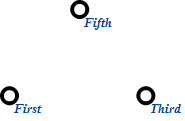
\includegraphics{images/4/gen/gen5_f_a_f_a_f_before}
  \caption{Содержимое sc-сегмента segment после генерации третьего sc-узла ла}
  \label{fig:gen5_f_a_f_a_f_before}
\end{figure}

В классе \lstinline|sc_session| есть специальный метод
\lstinline|gen5_f_a_f_a_f|, который генерирует второй и четвертый
элементы пятиэлементной sc-конструкции, если известны ее первый,
третий и пятый элементы. Его сигнатура выглядит следующим образом:

\begin{lstlisting}[texcl]
class sc_session
{
public:
    // $\dots$
    virtual sc_retval gen5_f_a_f_a_f(
        // sc-адрес 1-го элемент
        sc_addr e1,

        // по этому адресу поместить sc-адрес 2-го элемент
        sc_addr *e2,

        // sc-сегмент, в котором будет сгенерирован 2-ой элемент
        sc_segment *seg2, 

        // тип 2-го элемента
        sc_type t2,

        // sc-адрес 3-го элемент
        sc_addr e3,

        // по этому адресу поместить sc-адрес 4-го элемент
        sc_addr *e2,

        // sc-сегмент, в котором будет сгенерирован 4-ой элемент
        sc_segment *seg4,

        // тип 4-го элемента
        sc_type t4,

        // sc-адрес 5-го элемент
        sc_addr e5
    ) = 0;
    // $\dots$
};
\end{lstlisting}

Генерацию пятиэлементной sc-конструкции с sc-узлами \vidtf{First},
\vidtf{Third}, \vidtf{Fifth} можно провести следующим образом:

\begin{lstlisting}[texcl]
// переменная для sc-адреса 2-го элемента пятиэлементной sc-конструкции.
sc_addr e2 = 0;

// переменная для sc-адреса 4-го элемента пятиэлементной sc-конструкции.
sc_addr e4 = 0;

// Генерация sc-дуги между 1-ым и 3-им, 5-ым и 2-ым элементами.
session->gen5_f_a_f_a_f(
    // 1-ый элемент
    e1,

    // в e2 будет помещен sc-адрес 2-го элемента
    &e2,

    // sc-сегмент, в котором будет сгенерирован 2-ой элемент
    segment,

    // тип 2-ого элемента - константная позитивная sc-дуга
    SC_A_CONST|SC_POS,

    // 3-ий элемент
    e3,

    // в e4 будет помещен sc-адрес 4-го элемента
    &e4,

    // sc-сегмент, в котором будет сгенерирован 4-ой элемент
    segment,

    // тип 4-ого элемента - константная позитивная sc-дуга
    SC_A_CONST|SC_POS,

    // 5-ий элемент
    e5
);
\end{lstlisting}

После выполнения приведенного выше куска кода состояние sc-сегмента
будет таким, как показано на рис.~\ref{fig:gen5_f_a_f_a_f_after}.

Метод \lstinline|sc_session::gen5_f_a_f_a_f| работает аналогично
методу \lstinline|sc_session::gen3_f_a_f|, поэтому для него
справедливо все сказанное ранее про
\lstinline|sc_session::gen3_f_a_f|.

\begin{figure}
  \centering
  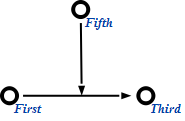
\includegraphics{images/4/gen/gen5_f_a_f_a_f_after}
  \caption{Пример генерации пятиэлементной sc-конструкции}
  \label{fig:gen5_f_a_f_a_f_after}
\end{figure}

\subsection{Работа с содержимым sc-элементов}

Каждому sc-элементу в программной модели sc-памяти может быть
установлено содержимое следующих типов (\lstinline|enum TCont| из
заголовочного файла \verb|sc_content.h|):
\begin{itemize}
\item строковое (\lstinline|TCSTRING|);
\item целочисленное (\lstinline|TCINT|);
\item вещественное (\lstinline|TCREAL|);
\item бинарное (\lstinline|TCDATA|);
\item отложенное (\lstinline|TCLAZY|);
\item пустое (\lstinline|TCEMPT|).
\end{itemize}

Для представления содержимого используется класс \lstinline|Content| (объявлен в
файле \verb|sc_content.h|), а для получения содержимого sc-элемента
предназначен метод \lstinline|sc_session::get_content|:

\begin{lstlisting}[texcl]
Content content = session->get_content(e1);

// Изначально у sc-элемента содержимое является пустым
if (content.type() == TCEMPTY) {
    // У sc-элемента пустое содержимое
}
\end{lstlisting}

В приведенном выше примере используется метод
\lstinline|Content::type|, который возвращает тип содержимого через
значение \lstinline|TCont|. Для установки содержимого sc-элементу
необходимо использовать метод \lstinline|sc_session::set_content| и
статические методы \lstinline|Content::integer|,
\lstinline|Content::real|, \lstinline|Content::string|,
\lstinline|Content::data|:
\begin{lstlisting}[texcl]
// Установка содержимого типа TCINT
session->set_content(first_el, Content::integer(1));

// Установка содержимого типа TCREAL
session->set_content(first_el, Content::real(0.05));

// Установка содержимого типа TCSTRING
session->set_content(first_el, Content::string("Hello world!!!"));

int my_data[] = { 1, 2, 3, 4, 5 };
// Установка содержимого типа TCDATA
session->set_content(first_el, Content::data(sizeof(my_data), my_data));
\end{lstlisting}

Чтобы получить доступ к данным объекта класса \lstinline|Content|
необходимо использовать \lstinline|union Cont|. Для пояснения я
продемонстрирую реализацию функции вывода на консоль содержимого
sc-элемента:
\begin{lstlisting}[texcl]
sc_retval print_content(const Content &content)
{
    // Класс Content имеет перегруженный оператор
    // приведения к типу Cont, поэтому возможна следующая запись:
    Cont c = cont;

    switch (cont.type()) {
    case TCSTRING:
        std::cout << c.d.ptr;
        break;
    case TCINT:
        std::cout << c.i;
        break;
    case TCREAL:
        std::cout << (double) c.r;
        break;
    case TCDATA:
        std::cout.write(c.d.ptr, c.d.size);
        break;
    case TCEMPTY:
        break;
    default:
        return RV_ERR_GEN;
    }

    return RV_OK;
}
\end{lstlisting}

Напоследок хочу сказать, что существует еще метод
\lstinline|sc_session::erase_content|, который уничтожает текущее
содержимое sc-элемента. После применения метода
\lstinline|sc_session::erase_content| sc-элемент будет иметь пустое
содержимое.

\subsection{Поиск в sc-памяти}
\subsubsection{Базовые механизмы поиска по шаблону}

Поиск в sc-памяти происходит по специальным шаблонам, которые
называются ограничениями (constraint). Для перебора конкретных
результатов поиска используется реализация идеи итераторов через
интерфейс \lstinline|sc_iterator|, объявленный в заголовочном файле
\verb|sc_iterator.h|:
\begin{lstlisting}[texcl]
/// Интерфейс итератора по различным видам sc-конструкций.
class sc_iterator
{
public:
    /// Переводит итератор на следующий результат поиска.
    virtual sc_retval next() = 0;

    /// @return true, если нет sc-конструкции, к которой можно перейти.
    /// @return false - в противном случае.
    virtual bool is_over() = 0;

    /// @return sc-адрес sc-элемента с порядковым номером @p num
    /// в найденной sc-конструкции.
    virtual sc_addr value(sc_uint num) = 0;

    virtual ~sc_iterator();
};
\end{lstlisting}

Для того чтобы понять как осуществлять поиск в sc-памяти ниже мы будем
рассматривать поиск в sc-памяти по различным видам ограничений. Первые
ограничения, на которые мы обратим своё внимание, будут ограничения
вида \lstinline|CONSTR_3_*_*_*|, которые используются для поиска трехэлементных
sc-конструкций. Ограничения \lstinline|CONSTR_3_*_*_*| бывают следующие:
\begin{itemize}
\item \lstinline|CONSTR_3_f_a_a|
\item \lstinline|CONSTR_3_f_a_f|
\item \lstinline|CONSTR_3_a_a_f|
\end{itemize}

Первое, что бросается в глаза в приеденных выше названиях, это
странный набор букв <<a>> и <<f>>. Рассмотрим
\lstinline|CONSTR_3_f_a_a| в качестве примера. Этот вид ограничения
используется для поиска трехэлементных sc-конструкций, а, как вы уже
знаете, элементы таких sc-конструкций пронумерованы. Поэтому первая
буква <<f>> в названии вида ограничения расшифровывается как
английское слово <<fixed>> и обозначает то, что 1-ый элемент
трехэлементной sc-конструкции известен. Вторая и третья буквы <<a>> в
названии вида ограничения расшифровываются как английское слово
<<assign>> и обозначают то, что 2-ой и 3-ий элементы неизвестны, и их
необходимо найти.

Посмотрим, как будет производиться поиск по такому виду
ограничения. Для этого допустим, что содержимое одного из sc-сегментов
как показано на рис.~\ref{fig:Data_for_CONSTR_3_f_a_a}. Так как поиск
проходит в рамках sc-сессии, то этот sc-сегмент должен быть открыт в
нашей sc-сессии.

\begin{figure}[h!]
  \centering
  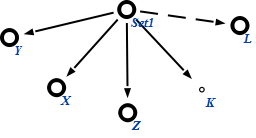
\includegraphics{images/4/search/Data_for_CONSTR_3_f_a_a}
  \caption{Содержимое sc-сегмента для поиска по \lstinline|CONSTR_3_f_a_a|}
  \label{fig:Data_for_CONSTR_3_f_a_a}
\end{figure}

Нам надо найти все константные sc-узлы, связанные константными
позитивными sc-дугами с известным sc-узлом \vidtf{Set1}. В этом случае
ограничения вида \lstinline|CONSTR_3_f_a_a| параметризируется
следующим образом:
\begin{enumerate}
\item sc-адрес sc-узла \vidtf{Set1};
\item \lstinline+SC_A_CONST|SC_POS+ (тип константной позитивной sc-дуги);
\item \lstinline+SC_CONST|SC_NODE+ (тип константного sc-узла).
\end{enumerate}

Как вы возможно уже догадались, если параметр для вида ограничения
фиксирован (fixed), то необходимо передавать sc-адрес, если параметр
не фиксирован (assign), то необходимо передавать шаблон-маску
\lstinline|sc_type| для поиска. Для формирования шаблона-маски
\lstinline|sc_type| нужно применять правило <<Чем меньше признаков
задано, тем больше будет найдено>>. Посмотрим на примерах, как
реализуется это правило:
\begin{itemize}
\item \lstinline|SC_EMPTY| или \lstinline|0|: под такую маску подойдет
  любой sc-элемент;
\item \lstinline|SC_NODE|: под такую маску подойдет любой sc-узел;
\item \lstinline+SC_ARC|SC_POS+: под такую маску подойдет любая
  позитивная sc-дуга;
\end{itemize}

Вернемся к нашему примеру. Следующий код выведет на консоль
идентификаторы всех константных sc-узлов, которые связаны с sc-узлом
\idtf{Set1} константной позитивной sc-дугой:
\begin{lstlisting}[texcl]
// Создаем итератор при помощи
// метода \verb|sc_session::create_iterator|
sc_iterator *it = session->create_iterator(
    // Создаем ограничение вида \verb|CONSTR_3_f_a_a|
    sc_constraint_new(
        CONSTR_3_f_a_a,    // вид ограничения
        Set1,              // 1-ый параметр
        SC_A_CONST|SC_POS, // 2-ой параметр
        SC_CONST|SC_NODE   // 3-ий параметр
    ),

    // Указываем, что итератор удалит ограничение
    // Здесь всегда указывайте true
    true
);

// Типичный цикл по результатам поиска
while (!it->is_over()) {

    // !!!! \color{red}{ОБРАТИТЕ ВНИМАНИЕ}:
    // !!!! Индексация с использованием метода
    // !!!! \verb|sc_iterator::value| работает как в массивах, т.е. с \verb|0|

    // Получаем 1-ый элемент найденной sc-конструкции
    // Им всегда будет sc-узел Set1
    sc_addr first = it->value(0);

    // Получаем 2-ой элемент найденной sc-конструкции
    sc_addr second = it->value(1);

    // Получаем 3-ий элемент найденной sc-конструкции
    sc_addr third = it->value(2);

    // Вывод строки на консоль
    std::cout << session->get_idtf(first) << " -> "
        << session->get_idtf(third)  << "\n";

    // Перевод итератора к следующей найденной sc-конструкции
    it->next();
}

// !!!! \color{red}{ОБРАТИТЕ ВНИМАНИЕ}:
// Надо обязательно освободить память, выделенную под итератор
delete it;
\end{lstlisting}

Приведенный выше код в результате своего исполнения выведет на консоль
(порядок может быть другим):
\begin{verbatim}
Set1 -> Y
Set1 -> X
Set1 -> Z
\end{verbatim}

В этом коде я применил следующие незнакомые для вас функции и методы:
\begin{itemize}
\item метод \lstinline|sc_session::create_iterator| для создания
  итератора по sc-конструкциям, подходящим под ограничение;
\item функцию \lstinline|sc_constraint_new| для создания ограничения
  определенного вида. Эта функция принимает неопределенное число
  аргументов, но первым аргументом всегда должна быть константа,
  которая задает вид ограничения.
\end{itemize}

На основе приведенного примера мы можем построить типовой код для
работы с объектами класса \lstinline|sc_iterator|. При помощи цикла
\lstinline|while| это можно сделать следующим образом:
\begin{lstlisting}[texcl]
// Создание итератора.
sc_iterator *it = session->create_iterator(
    sc_constraint_new(
        /* Здесь должны быть параметры ограничения. */
    ),
    true
);

while (!it->is_over()) {
    // Получение элементов найденной sc-конструкции
    // при помощи метода \verb|sc_iterator::value|.

    // Обработка результатов поиска.

    // Перевод итератора на следующий результат поиска.
    it->next();
}

// Обязательно нужно освободить память.
delete it;
\end{lstlisting}

Приведенный выше код можно переписать при помощи цикла \lstinline|for|
(блок создания итератора не приведен):
\begin{lstlisting}[texcl]
for (; !it->is_over(); it->next()) {
    // Получение элементов найденной sc-конструкции
    // при помощи метода \verb|sc_iterator::value|.

    // Обработка результатов поиска.
}

// Обязательно нужно освободить память.
delete it;
\end{lstlisting}

Однако два предыдущих варианта можно переписать в более простой форме
с использованием специального макроса \lstinline|sc_for_each| (блок
создания итератора не приведен):
\begin{lstlisting}[texcl]
sc_for_each (it) {
    // Получение элементов найденной sc-конструкции
    // при помощи метода \verb|sc_iterator::value|.

    // Обработка результатов поиска.
}

// Память освобождать не нужно, потому что она была освобождена
// при выходе из цикла \verb|sc_for_each|.
\end{lstlisting}

Обратите внимание, что в приведенном выше цикле макрос
\lstinline|sc_for_each| берет на себя следующую работу:
\begin{itemize}
\item проверка действительности итератора (вызов метода
  \lstinline|sc_iterator::is_over|);
\item перевод итератора на следующий результат поиска (вызов метода
  \lstinline|sc_iterator::next|);
\item освобождение памяти, на которую указывает \lstinline|it|, при
  выходе из цикла.
\end{itemize}

Цикл \lstinline|sc_for_each| работает так же, как и циклы
\lstinline|while| и \lstinline|for|, и поддерживает инструкции
\lstinline|break| и \lstinline|continue|.  А теперь перейдем к
рассмотрению других видов ограничений поиска, которые предоставляет
библиотека libsc.

Аналогично ограничениям вида \verb|CONSTR_3_*_*_*| существуют
ограничения вида \verb|CONSTR_5_*_*_*_*_*| для пятиэлементных
sc-конструкций. Ограничения \verb|CONSTR_5_*_*_*_*_*| бывают следующих
видов:
\begin{itemize}
\item \lstinline|CONSTR_5_f_a_a_a_a|
\item \lstinline|CONSTR_5_f_a_a_a_f|
\item \lstinline|CONSTR_5_f_a_f_a_a|
\item \lstinline|CONSTR_5_f_a_f_a_f|
\item \lstinline|CONSTR_5_a_a_a_a_f|
\item \lstinline|CONSTR_5_a_a_f_a_a|
\item \lstinline|CONSTR_5_a_a_f_a_f|
\end{itemize}

Работать с такими ограничениями надо так же, как и с ограничениями
вида \verb|CONSTR_3_*_*_*|.  Существует еще вид ограничения
\lstinline|CONSTR_3l2_f_a_a_a_f| для поиска sc-конструкций, одна из
которых показана на рис.~\ref{fig:CONSTR_3l2}. На
рис.~\ref{fig:CONSTR_3l2} элементы специально занумерованы.

\begin{figure}
  \centering
  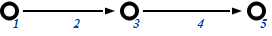
\includegraphics{images/4/search/CONSTR_3l2}
  \caption{ Пример sc-конструкции для ограничения вида
    \lstinline|CONSTR_3l2_f_a_a_a_f|}
  \label{fig:CONSTR_3l2}
\end{figure}

Хочу сказать еще про один вид ограничения, который называется
\lstinline|CONSTR_ORD_BIN_CONN1| и используется для поиска связки бинарного
отношения с фиксированным компонентом. На рисунке 2.19 показана
типовая sc-конструкция для поиска по этому виду ограничения. Элементы
с порядковыми номерами 1, 7 и 10 фиксированы, а для всех остальных
задается маска типа.

\begin{figure}
  \centering
  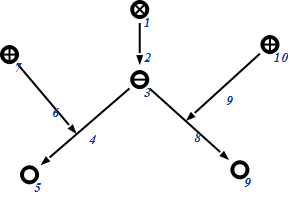
\includegraphics{images/4/search/CONSTR_ORD_BIN_CONN1}
  \caption{ Пример sc--конструкции для ограничения вида
    \lstinline|CONSTR_ORD_BIN_CONN1|}
  \label{fig:CONSTR_ORD_BIN_CONN1}
\end{figure}

\subsubsection{Oneshot-поиск по шаблону}

Oneshot-поиск - это поиск при помощи ограничения, при котором
находятся не все возможные sc-конструкции, а только одна (первая
найденная). При двух последовательных oneshot-поисках не
гарантируется, что будет найдена одна и та же sc-конструкция. Для
oneshot-поиска применяется специальная функция
\lstinline|search_oneshot|. Следующий код найдет sc-узел \idtf{L} и
входящую в него из sc-узла \idtf{Set1} переменную позитивную sc-дугу
(см. рис.~\ref{fig:Data_for_CONSTR_3_f_a_a}):
\begin{lstlisting}[texcl]
sc_addr first = 0, second = 0, third = 0; 
if (search_oneshot(session,
            sc_constraint_new(
                CONSTR_3_f_a_a,
                Set1,
                SC_ARC|SC_VAR|SC_POS,
                SC_CONST|SC_NODE
            ),
            // Указываем, что экземпляр ограничения необходимо удалить
            true,

            // Количество получаемых значений
            3,

            // Порядковый номер в ограничении 1-го результата
            0,
            // 1-ый элемент найденной конструкции - узел Set1
            &first,
            
            // Порядковый номер в ограничении 2-го результата
            1,
            // 2-ой элемент найденной конструкции –
// константная позитивная sc-дуга
            &second,

            // Порядковый номер в ограничении 3-го результата
            2,
            // 3-ий элемент найденной конструкции –
// константный sc-узел L
            &third
            ) == RV_OK) {
        // Результат найден
    } else {
        // Ничего не найдено
    }
\end{lstlisting}

Синтаксис \lstinline|search_oneshot| громоздок, поэтому для часто
используемых oneshot-поисков созданы специальные функции:

\begin{itemize}
\item Функция \lstinline|search_3_f_cpa_f|: поиск при помощи
  \lstinline|CONSTR_3_f_a_f|, когда для второго элемента задана маска
  типа \lstinline+SC_A_CONST|SC_POS+
\begin{lstlisting}[texcl]
// В эту переменную будет занесен
// sc-адрес найденного 2-го элемента
sc_addr e2 = 0;

if (search_3_f_cpa_f(session,
       // 1-ый элемент известен
       e1,

       // Если что-то будет найдено, то
       // переменная second получит в качестве значения sc-адрес
       // найденного sc-элемента
       &e2,

       // 3-ий элемент известен
       third
    ) == RV_OK) {
    // Поиск успешен
} else {
    // Поиск неуспешен
}
\end{lstlisting}

\item Функция \lstinline|search_3_f_cpa_cna|: поиск при помощи
  \lstinline|CONSTR_3_f_a_a|, когда для второго элемента задана маска
  типа \lstinline+SC_A_CONST|SC_POS+, а для третьего -
  \lstinline+SC_CONST|SC_NODE+
\begin{lstlisting}[texcl]
// В эту переменную будет занесен sc-адрес найденного 2-го элемента
sc_addr e2 = 0;

// В эту переменную будет занесен sc-адрес найденного 3-го элемента
sc_addr e3 = 0;

if (search_3_f_cpa_cna(session,
       // 1-ый элемент известен
       e1,

       // Если что-то будет найдено в качестве 2-го элемент, то
       // переменная second получит в качестве значения sc-адрес
       // найденного sc-элемента
       &e2,

       // Если что-то будет найдено в качесте 3-го элемент, то
       // переменная third получит в качестве значения sc-адрес
       // найденного sc-элемента
       &e3
   ) == RV_OK) {
   // Поиск успешен
} else {
   // Поиск неуспешен
}
\end{lstlisting}

\item Функция \lstinline|search_5_f_cpa_a_cpa_f|: поиск при помощи
  \lstinline|CONSTR_5_f_a_a_a_f|, когда для 2-го элемента задана маска
  типа \lstinline+SC_A_CONST|SC_POS+, для 3-го - \lstinline|SC_EMPTY|
  (нет ограничения на тип), для 4-го - \lstinline+SC_A_CONST|SC_POS+

\begin{lstlisting}[texcl]
// В эту переменную будет занесен sc-адрес найденного 2-го элемента
sc_addr e2 = 0;

// В эту переменную будет занесен sc-адрес найденного 3-го элемента
sc_addr e3 = 0;

// В эту переменную будет занесен sc-адрес найденного 4-го элемента
sc_addr e4 = 0;

if (search_5_f_cpa_a_cpa_f(
        session,
        e1,   // sc-адрес изввестен
        &e2,
        &e3,
        &e4,
        e5    // sc-адрес известен
        ) == RV_OK) {
    // Поиск успешен
} else {
    // Поиск неуспешен
}
\end{lstlisting}

\item Функция \lstinline|search_5_f_cpa_сna_cpa_f|: аналогично функции
  \lstinline|search_5_f_cpa_сna_cpa_f|, только для 3-го элемента
  задана маска типа \lstinline+SC_NODE|SC_CONST+

\item Функция \lstinline|search_3l2_f_a_a_a_f|: поиск при помощи
  \lstinline|CONSTR_3l2_f_a_a_a_f| (функция используется так же, как и
  все описанные выше oneshot-функции)
\end{itemize}

\subsection{Высокоуровневая работа с основными абстракциями в sc-памяти}

В данном разделе будут рассмотрены функционал, который упрощает и
делает более читабельными создание и обработку основных более
высокоуровневых конструкций, который встречаются в sc-памяти.

\subsubsection{Работа с sc-множествами}

Под sc-множеством в этом разделе подразумевается sc-узел,
т.е. sc-элемент, из которого могут выходить sc-дуги принадлежности
(позитивные, негативные и константные sc-дуги). Если sc-элемент входит
в sc-множество, значит от sc-множества к нему проведена позитивная
sc-дуга.

В заголовочном файле \verb|sc_set.h| объявлен класс
\lstinline|sc_set|, который предоставляет статические методы обработки
sc-множеств. Все статические методы собраны в класс
\lstinline|sc_set|, а не объявлены как функции, потому что в языке С++
класс предоставляет возможности пространства имен, когда не подходит
использование явного введения пространства имен с использование
объявления \lstinline|namespace|. Поэтому класс \lstinline|sc_set|
является классом только с формальной точки зрения.

В классе \lstinline|sc_set| собраны основные часто используемые операции по
обработки sc-множеств и они все в качестве первого аргумента принимают
sc-сессию, через которую будет осуществляться работа. Например, если
вам надо проверить пусто ли sc-множество, то при помощи метода
\lstinline|sc_set::is_empty| это можно сделать вот так:

\begin{lstlisting}[texcl]
#include <sc_set.h>

if (sc_set::is_empty(session, set1)) {
    // Множество пусто
} else {
    // Множество непусто
}
\end{lstlisting}

Первым мы рассмотрим набор статических методов, которые занимаются
проверкой вхождения sc-элемента в sc-множество. Таких методов
существует три вида:
\begin{lstlisting}[texcl]
/// Если sc-элемент c sc-адресом @p el входит в
/// sc-множество с sc-адресом @p set, то метод вернет
/// sc-адрес позитивной sc-дуги, связывающей
/// sc-множество с этим sc-элементом. В противном случае
/// метод вернет 0.
static sc_addr is_in(sc_session *s, sc_addr el, sc_addr set);

/// Если sc-элемент c sc-адресом @p el входит в
/// sc-множество с sc-адресом @p set1 или в sc-множество с sc-адресом
/// @p set2, то метод вернет sc-адрес позитивной sc-дуги, связывающей
/// sc-множество с этим sc-элементом, которое в списке аргументов стоит
/// раньше. В противном случае метод вернет 0.
static inline sc_addr is_in_any(sc_session *s, sc_addr el, sc_addr set1,
    sc_addr set2);

/// Если sc-элемент c sc-адресом @p el входит в
/// sc-множество с sc-адресом @p set1 и в sc-множество с sc-адресом
/// @p set2, то метод вернет true.
/// В противном случае метод вернет false.
static inline bool is_in_all(sc_session *s, sc_addr el, sc_addr set1,
    sc_addr set2);
\end{lstlisting}

Существуют варианты методов \lstinline|sc_set::is_in_any| и
\lstinline|sc_set::is_in_all|, которые перегружены для поддержки
большего количества sc-множеств (до 9 включительно). Я думаю, что
читателю должно быть понятно, как изменяется поведение методов при
использовании более двух sc-множеств. Самым часто используемым
является метод \lstinline|sc_set::is_in|.

Следующий набор статических методов предназначен для включения
sc-элемента в sc-множество:
\begin{lstlisting}[texcl]
/// Метод включает sc-элемент с sc-адресом @p el
/// в sc-множество с sc-адресом @p set1. Позитивная sc-дуга создается
/// в sc-сегменте @p seg. Признак константности этой sc-дуги
/// определяется исходя из константности sc-множества.
///
/// Есть варианты этого метода, которые перегружены для работы с более
/// чем одним sc-множеством (до 9 sc-множеств).
static inline sc_addr include_in(sc_session *s, sc_segment *seg,
    sc_addr el, sc_addr set1);

/// Метод работает аналогично \verb|sc_set::include_in|, только
/// позитивная sc-дуга создается в sc-сегменте включаемого sc-элемента.
///
/// Есть варианты этого метода, которые перегружены для работы с более
/// чем одним sc-множеством (до 9 sc-множеств).
static inline sc_addr include_in(sc_session *s, sc_addr el,
    sc_addr set1);

/// Метод включает в sc-множество с sc-адресом @p set1
/// sc-элемент с sc-адресом @p el1. Позитивная sc-дуга создается
/// в sc-сегменте @p seg. Признак константности этой sc-дуги
/// определяется исходя из константности sc-множества.
///
/// Есть варианты этого метода, которые перегружены для работы с более
/// чем одним включаемым sc-элементом (до 9 sc-множеств).
static inline void include(sc_session *s, sc_segment *seg, sc_addr set,
    sc_addr el1);

/// Метод работает аналогично \verb|sc_set::include|, только
/// позитивная sc-дуга создается в sc-сегменте sc-множества.
///
/// Есть варианты этого метода, которые перегружены для работы с более
/// чем одним включаемым sc-элементом (до 9 sc-множеств).
static inline void include(sc_session *s, sc_addr set, sc_addr el1);
\end{lstlisting}

И последний рассматриваемый набор статических методов предназначен для
исключения sc-элемента из sc-множества:
\begin{lstlisting}[texcl]
/// Исключает sc-элемент с sc-адресом @p el из
/// sc-множества с sc-адресом @p set1. Этот метод удаляет
/// позитивную sc-дугу, связывающую sc-множество с его элементом.
/// Если удаление sc-дуги произошло, то метод вернет true, иначе false.
///
/// Метод работает с sc-множествами без кратных вхождений элементов.
///
/// Есть варианты этого метода, которые перегружены для исключения
/// с более чем из одного sc-множества (до 9 sc-множеств). В этом случае
/// метод вернет true, если исключение произошло хотя бы из одного
/// sc-множества.
static inline bool exclude_from(sc_session *s, sc_addr el,
    sc_addr set1);

/// Этот метод почти аналогичен методу \verb|sc_set::exclude_from|, только
/// он учитывает кратные вхождения элемента в sc-множество.
static inline bool exclude_multi_from(sc_session *s, sc_addr el,
    sc_addr set1);

/// Удаляет элементы sc-множества с sc-адресом @p set.
static void erase_from(sc_session *s, sc_addr set);
\end{lstlisting}

\subsubsection{Работа с sc-связками}

Класс \lstinline|sc_tup| (объявлен в файле \verb|sc_tuple.h|)
предоставляет статические методы для работы с sc-связками. Самой
распространенной операцией над sc-связкой является получение компонент
с указанным атрибутом. Для этого можно использовать oneshot-поиск,
однако удобнее пользоваться статическим методом
\lstinline|sc_tup::at|. Например, вот так:
\begin{lstlisting}[texcl]
#include <sc_tuple.h>

// $\dots$

sc_addr first_component = sc_tup::at(
    session,
    tuple,   // sc-адрес связки
    N1_      // sc-адрес атрибута \verb|1_|
);

// \verb|first_component| будет равно 0, если
// компонент с атрибутом \verb|1_| не был найден
if (first_component) {
    // Компонент найден
} else {
    // Компонент не найден
}
\end{lstlisting}

Также распространенной операцией является добавление в sc-связку
компонента с заданным атрибутом. Для этого можно использовать
низкоуровневые методы типа \lstinline|sc_session::gen5_f_a_f_a_f|, но, на мой
взгляд, гораздо удобнее использовать статический метод
\lstinline|sc_tup::add|. Вот два способа добавить компонент component с атрибутом
\idtf{1\_} в связку \lstinline|tuple|:
\begin{lstlisting}[texcl]
sc_tup::add(
    session,
    segment,  // все sc-дуги будут сгенерированы в этом sc-сегменте
    tuple,    // sc-адрес связки
    N1_,      // sc-адрес атрибута
    component // sc-адрес добавляемого компонента
);

// Все sc-дуги будут сгенерированы в sc-сегменте,
// в котором находится sc-элемент \verb|tuple|
sc_tup::add(
    session,
    tuple,    // sc-адрес связки
    N1_,      // sc-адрес атрибута
    component // sc-адрес добавляемого компонента
);
\end{lstlisting}

\subsubsection{Работа с sc-отношениями}

Аналогично классам \lstinline|sc_set| и \lstinline|sc_tup| для работы
с sc-отношениями есть класс \lstinline|sc_rel|, объявленный в файле
\verb|sc_relation.h|. Часто используемыми операциями для работы с
sc-отношениями являются добавление бинарной ориентированной связки в
sc-отношение и поиск бинарной ориентированной связки с указанными
компонентами.

Для добавления бинарной ориентированной связки в sc-отношение
используется статический метод \lstinline|sc_rel::add_ord_tuple|:
\begin{lstlisting}[texcl]
/// Метод создает бинарную ориентированную sc-связку, в которую
/// включает под атрибутом \verb|1_| sc-элемент с sc-адресом @p v1, а
/// под атрибутом \verb|2_| - sc-элемент с sc-адресом @p v2.
/// Созданная sc-связка включается в sc-отношение @p rel.
/// SC-адрес созданной sc-связки возвращается в качестве результата.
///
/// Признак константности sc-связки определяется по константности
/// sc-отношения.
///
/// Если необходимы sc-дуги, связывающие sc-связку с ее компонентами,
/// то можно передать в качестве аргументов @p av1 и @p av2 адреса
/// переменных, в которые будут записаны sc-адреса соответствующих
/// sc-дуг. По-умолчанию в качестве этих аргументов передается 0.
static sc_addr add_ord_tuple(sc_session *s, sc_addr rel, sc_addr v1,
    sc_addr v2, sc_addr *av1=0, sc_addr *av2=0);
\end{lstlisting}

Для поиск бинарных ориентированных sc-связок в sc-отношении могут быть
использованы следующие статические методы класса \lstinline|sc_rel|:
\begin{lstlisting}[texcl]
/// В бинарном ориентированном sc-отношении с sc-адресом @p rel
/// находит связку, в которой компонентом с атрибутом \verb|1_| является
/// sc-элемент с sc-адресом @p val1.
///
/// Метод возвращает sc-адрес компонента с атрибтом \verb|2_| в данной связке.
/// Если такой связки не найдено, то метод вернет 0.
///
/// Если необходимо получить sc-адрес найденной связки, то в качестве
/// @p tuple можно передать адрес переменной, куда будет записан искомый
/// sc-адрес.
static inline sc_addr bin_ord_at_2(sc_session *s, sc_addr rel,
    sc_addr val1, sc_addr *tuple=0);

/// Этот метод аналогичен методу \verb|sc_rel::bin_ord_at_2|, только теперь
/// мы ищем связку, зная sc-адрес компонента с атрибутом \verb|2_|, а
/// возвращаем компонент с атрибутом \verb|1_|.
static sc_addr bin_ord_at_1(sc_session *s, sc_addr rel, sc_addr val2,
    sc_addr *tuple=0);
\end{lstlisting}

\subsubsection{Двусвязный список в sc-памяти}

Библиотека libsc предоставляет функционал для представления в
sc-памяти двусвязных списков. Для этого используются ключевые узлы
\idtf{list\_next\_} и \idtf{list\_value\_}, которые находятся в
sc-сегмент \verb|/proc/keynode|. На рис.~\ref{fig:Example_sc_list}
показан пример кодирования списка из константных sc-узлов \idtf{X},
\idtf{Y}, \idtf{Z}.

\begin{figure}
  \centering
  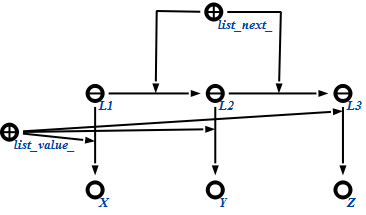
\includegraphics{images/4/Example_sc_list}
  \caption{Кодирование списка из элементов X, Y, Z}
  \label{fig:Example_sc_list}
\end{figure}


Элементы \idtf{L1}, \idtf{L2}, \idtf{L3} называются элементами списка
и имеют идентификаторы исключительно для наглядности
объяснения. Элемент \idtf{L1} – это начальный элемент списка, а
\idtf{L3} – конечный элемент списка. Каждый элемент списка является
связкой из двух компонентов:
\begin{itemize}
\item под атрибутом \idtf{list\_value\_} в элемент списка входит его
  значение. Например, на рис.~\ref{fig:Example_sc_list} значением
  элемента списка \idtf{L1} является sc-узел \idtf{X};
\item под атрибутом \idtf{list\_next\_} в элемент списка входит
  следующий элемент списка. Этот компонент связки может
  отсутствовать. Например, на рис.~\ref{fig:Example_sc_list} следующим
  для элемента списка \idtf{L1} является элемент списка \idtf{L2}, а
  для элемент списка \idtf{L3} нет следующего элемента, потому он
  является концевым.
\end{itemize}

По способу кодирования список, представленный на
рис.~\ref{fig:Example_sc_list}, является односвязным, но по интерфейсу
работы с ним является двусвязным. В заголовочном файле
\verb|sc_list.h| объявлен класс \lstinline|sc_list|, который
предоставляет статические методы для работы со списками в sc-памяти и
STL-совместимые однонаправленные итераторы для перебора их
элементов. Все методы класса \lstinline|sc_list| в качестве своего
первого аргумента принимают sc-сессию, через которую будет
производиться работа с sc-памятью.

Первым методом, который вы рассмотрим, будет
\lstinline|sc_list::create|. Он объявлен как:
\begin{lstlisting}[texcl]
/// Создать элемент списка в sc-сегменте @p seg со значением @p val и
/// установить его следующим для элемента @p prev
static sc_addr create(sc_session *s, sc_segment *seg, sc_addr val,
    sc_addr prev=0);
\end{lstlisting}

Метод \lstinline|sc_list::create| нужно использовать для создания
первого элемента списка следующим образом:
\begin{lstlisting}[texcl]
// Создание головы списка.
sc_addr list_head = sc_list::create(
    session,
    segment,
    value    // sc-адрес значения головы списка
);

// Список состоит из одного элемента, поэтому
// голова списка является и его концом.
sc_addr list_tail = list_head;
\end{lstlisting}

Либо метод можно использовать для добавления элемента в список, если
известен его конец:
\begin{lstlisting}[texcl]
// Создаем второй элемент списка.
// Созданный элемент будет концевым в нашем списке.
sc_addr list1 = sc_list::create(
    session,
    segment,
    value1    // sc-адрес значения этого элемента списка

    // sc-адрес элемента списка,
    // для которого созданный элемент будет следующим
    list_tail
);

// Запомним, что list1 - это конец списка.
list_head = list1;
\end{lstlisting}

Для работы со списками существует набор статических get-методов,
которые позволяют получить различные характеристики для элемента
списка:
\begin{lstlisting}[texcl]
/// Возвращает sc-адрес следующего элемент списка
/// для элемента списка @p list.
/// Вернет 0, если элемент списка @p list является хвостовым.
static sc_addr get_next(sc_session *s, sc_addr list);

/// Возвращает sc-адрес предыдущего элемент списка
/// для элемента списка @p list.
/// Вернет 0, если элемент списка @p list является головным.
static sc_addr get_prev(sc_session *s, sc_addr list);

/// Возвращает sc-адрес значения элемента списка @p list.
/// Вернет 0, если для элемента списка @p list значение не установлено.
static sc_addr get_value(sc_session *s, sc_addr list);
\end{lstlisting}

Так же в классе \lstinline|sc_list| существует набор статических
set-методов, которые позволяют установить различные характеристики для
элемента списка:
\begin{lstlisting}[texcl]
/// Установить следующим элементом для элемента списка @p list1
/// sc-элемент @p list2.
/// Необходимые sc-элементы будут созданы в sc-сегменте @p seg.
static sc_retval set_next(sc_session *s, sc_segment *seg, sc_addr list1,
    sc_addr list2);

/// Аналогично \verb|#sc_list::set_next|, только необходимые sc-элементы
/// будут созданы в sc-сегменте, в котором находится sc-элемент c
/// sc-адресом @p l1.
static inline sc_retval set_next(sc_session *s, sc_addr l1, sc_addr l2);

/// Установить значением для элемента списка @p list1
/// sc-элемент с sс-адресом @p list2.
/// Необходимые sc-элементы будут созданы в sc-сегменте @p seg.
static sc_retval set_value(sc_session *s, sc_segment *seg, sc_addr list,
    sc_addr val);

/// Аналогично \verb|#sc_list::set_value|, только необходимые sc-элементы
/// будут созданы в sc-сегменте, в котором находится sc-элемент @p l1.
static inline sc_retval set_value(sc_session *s, sc_addr l, sc_addr v);
\end{lstlisting}

Самый простой способ перебора элементов таких списков от головы к
хвосту можно организовать следующим образом:
\begin{lstlisting}[texcl]
// Текущим обрабатываемым элементом
// является голова списка.
sc_addr list_current = list_head;
while (list_current) {
    // Получаем значения текущего элемента списка.
    sc_addr value = sc_list::get_value(session, list_current);

    //
    // Производим обработку значения.
    //

    // Получаем следующий элемент списка для текущего.
    // Если текущим является хвостовой элемент, то
    // \verb|sc_list::get_next| вернет 0.
    list_current = sc_list::get_next(session, list_current);
}
\end{lstlisting}

Однако при помощи однонаправленных итераторов такой перебор элементов
списка можно организовать более лаконично:
\begin{lstlisting}[texcl]
// Создаем итератор, указывающий на голову списка.
sc_list::iterator list_it(session, list_head);

// Создаем итератор, который покажет, что
// достигнут конец списка.
sc_list::iterator list_it_end;

for (; list_it != list_it_end; ++list_it) {
    // Получаем значения текущего элемента списка.
    sc_addr value = *list_it;

    //
    // Производим обработку значения.
    //
}
\end{lstlisting}

Кроме \lstinline|sc_list::iterator| есть еще
\lstinline|sc_list::reverse_iterator|, который осуществляет перебор
списка в обратном направлении, т.е. оператор \verb|++| переводит итератор с
текущего элемента списка на предыдущий. Для определения начала списка
все равно необходимо использовать объект класса
\lstinline|sc_list::reverse_iterator|, созданный без аргументов.

И напоследок, если список вам уже не нужен, то его можно удалить при
помощи метода \lstinline|sc_list::erase|:
\begin{lstlisting}[texcl]
/// Удалит элемент списка по sc-адресу @p list
/// и все следующие за ним элементы списка.
/// Удаляет только элементы списка, а не их значения.
///
/// Как правило в качестве @p list
/// надо передавать головной элемент списка
static void erase(sc_session *s, sc_addr list);
\end{lstlisting}

%%% Local Variables: 
%%% mode: latex
%%% TeX-master: "main"
%%% End: 
